\chapter{Introduction}
Introduce what \LaTeX is.

At the beginning of most documents there will be information about the
document itself, such as the title and date, and also information about the
authors, such as name, address, email etc. All of this type of information
within LaTeX is collectively referred to as \textit{top matter}. 

\section{Definition}
Following conventions will be used in this report:  \\
\package{package}   \\
\command|command|   \\
\option{option}	    \\

%%%%%%%%%%%%%%%%%%%%%%%%%%%%%%%%%%%%%%%%%%%%%%%%%%%%%%%%%%%%%%%%%%%%%%%%
\section{Packages}
While writing your document, you will probably find that there are some
areas where basic LaTeX cannot solve your problem. If you want to include
graphics, colored text or source code from a file into your document, you
need to enhance the capabilities of LaTeX. Such enhancements are called
packages. Some packages come with the LaTeX base distribution. Others are
provided separately. Modern TeX distributions come with a large number of
packages pre-installed. 

%%%%%%%%%%%%%%%%%%%%%%%%%%%%%%%%%%%%%%%%%%%%%%%%%%%%%%%%%%%%%%%%%%%%%%%%
\section{Box}
The key lies in \LaTeX{} is box, which is the smallest unit processed by
\LaTeX{}. Everything is thought as a box, and then aligned into page.

%%%%%%%%%%%%%%%%%%%%%%%%%%%%%%%%%%%%%%%%%%%%%%%%
\subsection{Introduction}
A \emph{box} is the \TeX term for an invisible container that can hold a
visible element, nothing, or other boxes. \emph{Glue} is the \TeX term for
an invisible connector that determines the separation between boxes. A 
visible element can be a letter, image, geometric shape, etc. \TeX builds 
pages by gluing boxes together. In a typical document, letter boxes are glues 
to other letter boxes to form words, which are then elastically glued to 
other words to form sentences. Sentences are broken into lines and placed 
in paragraph boxes. Elastic glue is squeezed or stretched to fully justify 
lines within paragraph boxes. Paragraph boxes are glued to diagram boxes, 
and so on.
\begin{figure}[htp]
    \centering
    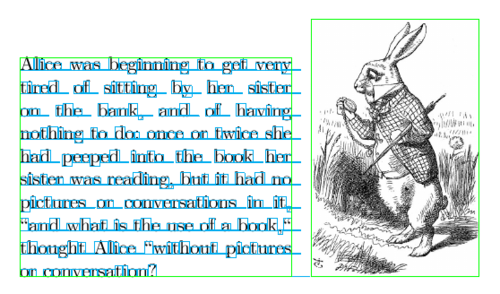
\includegraphics[scale=0.7]{500px-Latex_boxed_characters}
\end{figure}

While it is true that boxes can hold other boxes, not all commands that can 
generate boxes be used within all other commands that can generate boxes. 
There are often workarounds for these limitations.

The size of a box is typically to the size and position of its contents,
but it doesn't have to be. Many box commands accept custom widths and/or
heights, and there are other commands that effect the shape and position 
of boxes. Boxes are placed relative to other boxes, while visible elements
are placed relative to the boxes which contains them.
\begin{figure}[htp]
    \centering
    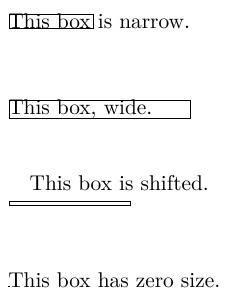
\includegraphics[scale=0.5]{LaTeX_boxes_that_dont_match_their_contents}
\end{figure}
%%%%%%%%%%%%%%%%%%%%%%%%%%%%%%%%%%%%%%%%%%%%%%%%
\subsection{Boxes}

%%%%%%%%%%%%%%%%%%%%%%%%
\subsubsection{character boxes}
\TeX character boxes have three dimensional propreties:
\begin{itemize}
    \item \textbf{height} is the length between the baseline and the top of the box.
    \item \textbf{depth} is the length between the baseline and the bottom of the box.
    \item \textbf{width} is the width of the box.
\end{itemize}
\begin{figure}[htp]
    \centering
    
\includegraphics[scale=0.7]{300px-charbox}
\end{figure}

%%%%%%%%%%%%%%%%%%%%%%%%
\subsubsection{parbox, minipage, and pbox}
A \command|\parbox| is a box of specific width formatted in paragraph mode. 
In paragraph mode, text is broken into lines and lines are broken into pages.
\command|\parbox[pos][height][contentpos]{width}{text}|

\option{width} defines the width of the paragraph box. Text will be broken 
into lines so that it fits within this width. 

\option{pos} selects which baseline to join. It can be \textbf{t}op, \textbf{b}ottom,
or \textbf{c}enter. 

\option{contentpos} positions the contents of the box within the box. It 
can be one of \textbf{c}enter, \textbf{t}op, \textbf{b}ottom or \textbf{s}pread. Note
that \option{contentpos} has no effect if the box is not larger than the
text it contains.


\command|\pbox[pos][height]{width}{text}|
